% !TEX TS-program = pdflatex
% !TEX encoding = UTF-8 Unicode

% This is a simple template for a LaTeX document using the "article" class.
% See "book", "report", "letter" for other types of document.

\documentclass[11pt]{article} % use larger type; default would be 10pt

\usepackage[utf8]{inputenc} % set input encoding (not needed with XeLaTeX)
\usepackage{amsmath}
\usepackage{graphicx}
\graphicspath{ {./} }
%%% Examples of Article customizations\textbf{}
% These packages are optional, depending whether you want the features they provide.
% See the LaTeX Companion or other references for full information.

%%% PAGE DIMENSIONS
\usepackage{geometry} % to change the page dimensions
\geometry{a4paper} % or letterpaper (US) or a5paper or....
% \geometry{margin=2in} % for example, change the margins to 2 inches all round
% \geometry{landscape} % set up the page for landscape
%   read geometry.pdf for detailed page layout information

\usepackage{graphicx} % support the \includegraphics command and options
\usepackage{physics}

% \usepackage[parfill]{parskip} % Activate to begin paragraphs with an empty line rather than an indent

%%% PACKAGES
\usepackage{booktabs} % for much better looking tables
\usepackage{array} % for better arrays (eg matrices) in maths
\usepackage{paralist} % very flexible & customisable lists (eg. enumerate/itemize, etc.)
\usepackage{verbatim} % adds environment for commenting out blocks of text & for better verbatim
\usepackage{subfig} % make it possible to include more than one captioned figure/table in a single float
\usepackage{fancyvrb}
\usepackage[hyphens]{url}
\usepackage{hyperref}
\usepackage{listings}



% These packages are all incorporated in the memoir class to one degree or another...

%%% HEADERS & FOOTERS
\usepackage{fancyhdr} % This should be set AFTER setting up the page geometry
\pagestyle{fancy} % options: empty , plain , fancy
\renewcommand{\headrulewidth}{0pt} % customise the layout...
\lhead{}\chead{}\rhead{}
\lfoot{}\cfoot{\thepage}\rfoot{}

%%% SECTION TITLE APPEARANCE
\usepackage{sectsty}
\allsectionsfont{\sffamily\mdseries\upshape} % (See the fntguide.pdf for font help)
% (This matches ConTeXt defaults)

%%% ToC (table of contents) APPEARANCE
\usepackage[nottoc,notlof,notlot]{tocbibind} % Put the bibliography in the ToC
\usepackage[titles,subfigure]{tocloft} % Alter the style of the Table of Contents
\renewcommand{\cftsecfont}{\rmfamily\mdseries\upshape}
\renewcommand{\cftsecpagefont}{\rmfamily\mdseries\upshape} % No bold!

%%% END Article customizations

%%% The "real" document content comes below...

\title{Mining Bitcoin Using Grover's Algorithm}


\author{Shazil Arif}
%\date{} % Activate to display a given date or no date (if empty),
         % otherwise the current date is printed 

\begin{document}
\maketitle

\tableofcontents

\section{Introduction}{}

In this paper we cover the basics of Bitcoin, Blockchain and Bitcoin's Proof-of-Work Consensus Algorithm and explore what mining is. We will discuss why mining is difficult and the existing solutions that exist for it. We will briefly discuss reversible computation and Unitary matrices. We will look at a Python solution to mine a block (at a very small scale) using Grover's Algorithm. Then we will discuss some practical limitations and scalability issues when implementing this in practice.\\


\noindent \textbf{Disclaimer:} I'm not an expert in any of the topics discussed in this paper.

\section{Blockchain}{}

A blockchain is simply a ledger. It records transactions. It records the sender, receiver and the amount being sent by the sender to the receiver. It's a concept that has been around for thousands of years.\\

\noindent In ancient times, in places like Babylon and Mesopotamia, people used clay tablets and carved details of transactions onto these tablets [2]. Slowly these evolved into papyrus documents. In the 15th century, Italian mathematician Luca Pacioli introduced the idea of double entry bookkeeping. It became the underlying principle of today's field of accounting. It's very simple, each transaction involves a credit entry for one party and a debit entry for another party.\\

\noindent Blockchain is essentially a modern version of a ledger. It is digital but also \textbf{decentralized}. We'll discuss the concept of decentralization more in depth but, at a high level what it means is that nobody owns or controls the ledger. In ancient times, ledgers were stored in temples, then banks in more modern times. Instead, the blockchain is stored on various computers referred to as a network.\\

\noindent Blockchain is in fact not tied to Bitcoin. It was invented years before Bitcoin by Stuart Haber and W. Scott Stornetta who worked at Bell labs in 1991. Their motivation was to create a way of making digital documents immutable and tamper-proof. \\

\noindent In technical terms, a blockchain is implemented as a distributed database. The database structures data into blocks and links them together, creating a chain of blocks. Each block contains a set of transactions and is assigned a hash. The hash is a combination of multiple details including sender, receiver, transactions etc.  but most importantly, the hash of the previous block. Each block contains the hash of the block before it. For example, Block 2 would have the hash of Block 1. This is important, because if someone tries to tamper with Block 1, it's hash would change but, Block 2 contains Block 1's hash which would also become invalid and a result, the hash of Block 2 would become invalid. If there are more blocks, Block 3, 4 and so on, all of them become invalid. This is very powerful as it makes a blockhain highly tamper proof. Attempting to tamper one block, invalidates all the others. \\

\section{Currency and Cryptocurrencies}{}
What is a cryptocurrency? How does it have value if I can't see or feel it? A question many people commonly ask.\\


\noindent Fundamentally, nowadays most currencies (digital or paper) have no value. It has value because society agreed that it will be used as a medium of exchange and a result, has value. It is a social construct. This is known as the Fiat Standard. It's worth pointing out that this wasn't always the case. Before 1971, the US dollar and many currencies around the world were backed gold, a physical asset. It was known as the Bretton Wood System or Agreement. However, in August 1971, President Richard Nixon broke this agreement in order to fight unemployment, inflation and stabilize the US dollar \cite{17}. The US dollar was no longer backed by gold and many other countries followed.\\


\noindent Most Cryptocurrencies (including Bitcoin) are also technically fiat currencies. They are not backed by anything and they only have value because the people using it agreed upon them as a medium of exchange. However, there are other factors that play a role in determining the value of a currency. We'll discuss these factors, specifically for Bitcoin in the next section. In addition, these currencies live on a Blockchain that is secured via cryptographic hash functions, which is where the name comes from. Cryptography + currency = Cryptocurrency\\

\section{Bitcoin}{}
\subsection{Overview}{}
As we discussed earlier, Bitcoin is a cryptocurrency. It was introduced to the world in the famous white paper titled \textbf{Bitcoin: A Peer-to-Peer Electronic Cash System} published by Satoshi Nakamoto on October 31, 2008, not long after the 2008 financial collapse. What Satoshi really wanted was: decentralized currency, one that was truly controlled by no bank or third party, instant online transfers, and make all of that secure.

\subsection{Price Factors}{}
What factors determine the price of Bitcoin? Why does it fluctuate? We can break this up into a few categories as follows:

\begin{itemize}
\item Supply
\item Demand
\item Competition
\item Regulatory and News Development
\end{itemize}

\subsubsection{Supply}{}
A scarce resource, generally has value. For example, Gold. Gold is limited in supply and is difficult to mine. Bitcoin is also limited in supply and is difficult to produce. There is a max number that can ever be mined, which is 21 million. New Bitcoin's are released into circulation by mining. However, over time the mining difficulty increases and the reward decreases. The reward is halved when 210,000 new blocks are added to the blockchain, which occurs roughly every 4 years. For example, on May 2020, the reward decreased from 12.5 BTC to 6.25 BTC. As the reward decreases, new Bitcoin's are released into circulation at a slower rate, this limited supply drives the value up. In fact, it has been observed that the price of Bitcoin hits new record prices roughly 1.5 years after a halving event [1].

\subsubsection{Demand}{}
The demand is mainly a function of adoption. A currency has more value when it is more widely adopted as a medium of exchange. As it becomes more mainstream, more people will demand it and with the limited supply, the price further goes up. As more countries adopt and accept Bitcoin as a legal tender, its value will increase.

\subsubsection{Competition and Implementation Technology}{}
When people have choice, they can pick. This is true for goods and also true for currencies. As more and more cryptocurrencies enter the market, the competition against Bitcoin continues to increase. For example, Ethereum is another very popular cryptocurrency. Many cryptocurrencies have different underlying protocols, design decisions, lower transactions fees, all these factors play a role in competing against Bitcoin. As more options become available, the demand would go down for Bitcoin and a result, the price would also decrease.

\subsubsection{Regulatory and News Development}{}
News surrounding the cryptocurrency space and Bitcoin plays a big role in the price. Most of the news has to do with regulatory and adoption developments. For example, when a country decides to adopt Bitcoin or when a country decided to ban it. Positive news increases the price and negative news decreases the price. For example, when the Securities Exchange Commission (SEC) announced crypto exchanges must register with an agency, the Bitcoin price dropped [6]. Or, when El Salvador decided to make Bitcoin a legal tender and bought several Bitcoins themselves, the price rose [5].

\subsection{What does Bitcoin solve?}{}
It's worth pointing out that Bitcoin did not solve the problem of online money transfers or creating tamper proof ledgers, these were solved problems before Bitcoin came around. Bitcoin drew heavily on earlier works such as Proof-of-Work and Blockchain technology. What Satoshi really solved was the double spending problem. He proposed a solution to this using a protocol known as \textbf{Proof-of-Work}. We will dive into more details about this, but, at a high level it involves a distributed network and each computer in the network must use CPU power to find a number (known as nonce) that produces a hash with a target number of leading zeros.
\subsection{The Bitcoin Network and Distributed Nodes}{}
What does distributed mean? What is a node? If you are familiar with Distributed Computation it will be easier to understand. However, if you are not, we'll attempt to explain it as best as possible. \\

\noindent A network is a set of computers. Each computer is called a node. These nodes can be in the same room or on completely opposite sides of the globe, this is the distributed part. So we have a set of computers all around the world, each has a copy of the blockchain. Each node also participates in the network by verifying transactions. Transactions are verified by solving the cryptographic hash puzzle and finding the nonce.
\subsection{Cryptography and Security}{}
Bitcoin uses the SHA-256 hashing algorithm. Each block is assigned a hash, it also stores the hash of the block before it. If any data in a block is changed, say the sender, receiver or a transaction, the hash is no longer valid and that block is also no longer valid and needs to be re-mined. Since other blocks also store the previous blocks hash, when a block is tampered with, all blocks after it are also invalidated because the previous blocks hash is invalid. This makes it very difficult to tamper with the blockchain, as one would have to re-mine multiple blocks, each of which requires immense computational effort.\\

\noindent Bitcoin also requires multiple confirmations per block. So let's say one node finds the nonce for a block, it requires atleast 6 other nodes to confirm the block [11]. This introduces additional security.\\

\noindent In the official Bitcoin whitepaper, the probability of an attacker succeeding is modelled as follows:\\

$1 - \sum_{k=0}^{z} \frac{ \lambda^{k} e^{-\lambda} } {k!} (1 - ({\frac{q}{p}}) ^ {(z-k)})$\\

Where $\lambda = z \frac{p}{q}$, $z$ is the number of blocks that need to be re-mined, $p$ is the probability that an honest node finds the next block and $q$ is the probability that the attacker finds the next block.\\

\noindent The specifics of the equation are not important, what's important is that the probability of the attack succeeding drops exponentially with the number of blocks $z$, which need to be re-mined. Safe to say, the Bitcoin blockchain is pretty secure.

\subsection{Public Adoption and Use Cases}{}
Bitcoin is yet to be widely adopted as a form of payment. However, it is slowly being adopted, especially in third world countries with weak currencies. For example, governments of countries like Venezuela and El Salvador have officially accepted Bitcoin as a form of payment. Even in first world countries, Bitcoin is becoming a popular form of digital payments. 


\section{Proof-of-Work and Mining}{}
\subsection{A brief history of Proof of Work}
Satoshi did not actually create Proof of Work. It was introduced by Adam Back in 1997 as a means of fighting email spam and Denial of Service Attacks (DoS) in web services [7]. The basic idea was that, before sending an email, the user's machine would have to do a small amount of computational work, say finding a number that produce a target hash and only then the email would be sent. In case of a spammer, for sending out mass emails, all that added computational work would not be possible for a single machine. Similar idea for preventing DoS attacks.

\subsection{Overview}

When a transaction occurs, it is not verified in real time, there is some delay. Before verification, these transactions are sent to a block. These unverified transactions are then verified by miners, whoever verifies it first, gets a reward. Miners (which are just computers in the network) verify the transaction by finding a number, known as nonce, which is ``Number only used once". It is essentially a number that produces the target hash for the block, which has a fixed number of zeros, in other words, it's our solution. The goal of mining is to find the nonce. When a miner verifies a block, it requires several other confirmations from other blocks (in case of an attacker). The current reward is 6.25 BTC, which is about \$305 USD. When this reward is paid out, new Bitcoin's are introduced into circulation, this is how Bitcoin's are produced.


\subsection{Mining Technology}
GPU's are a popular choice, thousands of these are clustered together to make mining rigs. ASIC's are also very popular, these are chips designed for the sole purpose of mining. Generally, buyers look for the best hash rate. Hash rate is the number of hashes that can be tried to find a nonce, per second. Nowadays, many ASIC's have hash rates above 1 TH/s [8], that is over a trillion hashes per second!
\subsection{Mining Difficulty}
Formally, the mining difficulty is defined using an equation. The specifics aren't that important but, essentially the difficulty depends on the required number of leading zeros. With each added zero, the difficulty increases exponentially [1].  The difficulty is adjused after every 2,016 blocks are added, which is roughly every 2 weeks. Bitcoin aims to add a new block to the blockchain roughly every 10 minutes, which is about 900 blocks per day. The mining difficulty is adjusted to maintain this rate [12].

\subsection{Environmental Impact of Mining}{}
Bitcoin mining requires immense computational resources. Many miners use GPU's and ASIC's to facilitate in mining. The mining difficulity has also increased millions of fold over time, which means more computational resources are required. For this reason, there are now mining pools, essentially groups of people that come together, combine their resources and share their reward, since the probability of succeeding individually is very low. There are mining rigs, which can be though of as data centers dedicated to mining bitcoin. This all means a large amount of electricty is consumed and lots of cooling is also required to keep the mining hardware cool. Some estimates have shown that Bitcoin mining consumes about 91 terrawatt-hours of electricity annually, which is more that what some countries consume [10]. For example, all of Finland consumes less electricity than Bitcoin.

\section{An Oracle for mining Bitcoin Blocks}{}

\subsection{Functions as Unitary Matrices}{}
We can represent a function as a Unitary Matrix. For example, suppose we have a reverse function that reverses the input bits.

\begin{center}
\begin{tabular}{ |c|c|c| } 
 \hline
 a & b & f = $ba$ \\ 
 0 & 0 & 00 \\ 
 0 & 1 & 10 \\ 
 1 & 0 & 01 \\ 
 1 & 1 & 11 \\ 
 \hline
\end{tabular}
\end{center}

We can represent this as a matrix as follows:\\

$
\begin{bmatrix}
& 00 & 01 & 10 & 11\\
00 &1 & 0 & 0 & 0\\
01 & 0 & 0 & 1 & 0\\
10 & 0& 1 & 0 & 0\\
11& 0& 0 & 0 & 1\\
\end{bmatrix}
$\\

\noindent The first row and column are simply labels. The way to interpret this is: 1 marks the answer. So you look at the column for a particular input, say 10 and then look for the row where there's a 1, the row number is the answer. For example, if we look at column 10, there is a 1 at row 01, meaning $f(10) = 01$

\subsection{Reversible Computing}{}
\noindent Quantum computation needs to be reversible. This means that for a given input, a circuit produces some output but, unlike classical computers, we should be able to recover the input from the output. Why is this a requirement?\\

\noindent Rolf Landauer proposed the Landauer principle, which proposes that \textbf{information is physical}. He proposed that fundamentally, logic gates dissipate heat because they are irreversible. Since they are irreversible, they \textbf{delete} information. He proposed that deleting a single bit of information increases a systems entropy and the associated energy is released as heat.\\

\noindent For example, a logical AND gate takes 2 inputs but produces only one output, we cannot recover the original bits, and so we lost or deleted information.  We can think of the information as being conserved, it can't be created or destroyed and so must go somewhere, and it dissipates away as heat.\\

\noindent Landauer proposed that the minimum amount of energy required to delete one bit of information was $K T$ ln (2), where K is the Boltzmann constant and T is the temperature of the system. It was derived from the Boltzmann Entropy Formula which states that $\frac{E}{T} = K ln(W)$ where $E$ is energy and $W$ is the number of states the system can be in. In the case of a bit, it can be in 2 states, 0 or 1 and so $W = 2$ and so we get $E = K T ln(2)$. For $N$ bits, we have $W = 2^{N}$ states which gives $E = K T ln(2^N)$ which is equivalent to $N K T ln (2)$ which shows that the energy dissipated by logic gates scales linearly with the number of bits.\\

\subsection{Reversible Functions}{}


\noindent We can turn an arbitrary non reversible function $f(x)$, into a reversible function by doing $U_{f} (x, h) = (x, h \oplus  f(x))$. \\

\noindent In terms of a matrix representing a function, we can ensure it is reversible by satisfying $U_f \ket{x} = (-1)^{f(x)} \ket{x}$\\

\noindent This means our diagonal contains -1 or 1. $f(x) = 0$ when $x$ is not a solution and $f(x) = 1$ when $x$ is a solution.

 \subsection{Pseudocode}{}
We can use the following Python pseudocode to create and use an oracle function for mining a bitcoin block:
\begin{Verbatim}[tabsize=4]
def f(x):	
	if x is a valid nonce:
		return 1
	return 0

def phase(x):
	return (-1)**f(x)

def functionToMatrix(fn, n):
	size = 2**n
	matrix = []
	for i in range(size):
		matrix[i][i] = fn(i)
	return matrix
	
\end{Verbatim} 

\section{Grover's Algorithm}{}
Grover's Algorithm is a quantum search algorithm. It can search an unsorted list of items in $O(\sqrt{N})$ evaluations of the oracle function, where $ N = 2^{n}$ possible states, where $n$ is the number of bits. It uses a technique called amplitude amplification that repeatedly applies the algorithm and with each iteration, our target result has a higher and higher probability of being the measured result [4]. Essentially, we are amplifying results of interest.\\

\noindent We start by defining a Unitary matrix $U_w$. Then we do the following:

\begin{itemize}

\item[1)] Initialize the system to the uniform superposition over all states:\\

$ \ket{s} = \frac{1}{\sqrt{N}}  \sum_{x = 0}^{N - 1} \ket{x}$

\item[2)] Perform the following $k$ times ($k$ is about $\frac{\pi}{4} \sqrt{N)}$:

\begin{itemize}
\item[1)] Apply the operator $U_w$
\item[2)] Apply the Grover diffusion operator $U_s = 2 \ket{s} \bra{s} - I$
\end{itemize}
\item[3)] Measure results
\end{itemize}

The circuit looks as follows:\\

\noindent 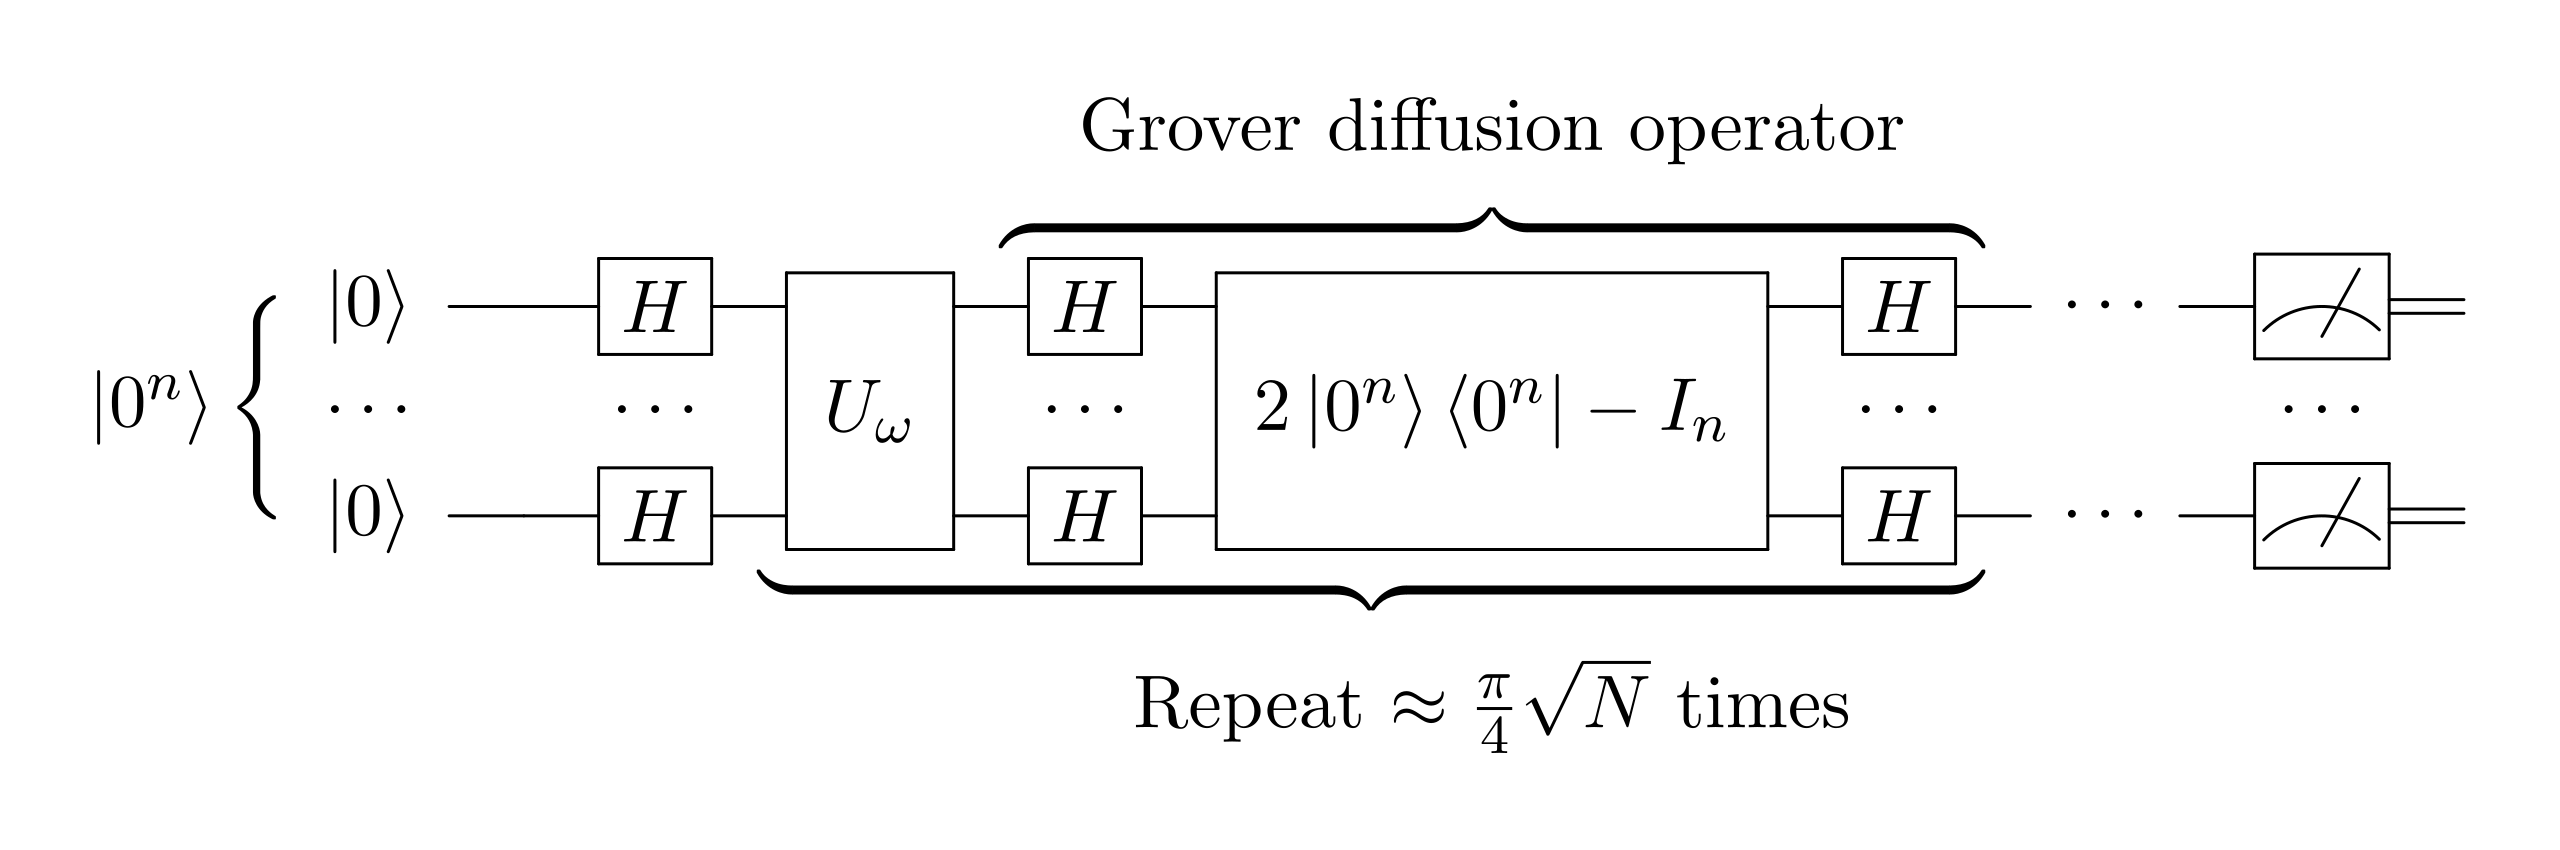
\includegraphics[keepaspectratio, width=15cm, height=15cm]{grover-circuit}

\section{Mining Implementation With Grover's Algorithm Overview}{}
We have implemented the full mining solution with Grover's Algorithm and tested it on a simulator and it works correctly. \\

\noindent From the official Bitcoin source code, we can see that a block is a 80 byte C++ structure that looks like this \cite{3}:

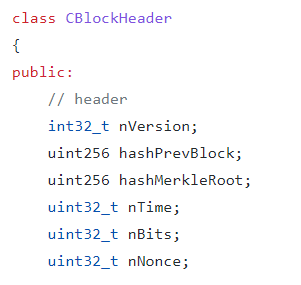
\includegraphics{block}

\noindent Based of this, we created a test block for our implementation. We used real numbers from block 2 of the Bitcoin Blockchain which can be found at \url{https://www.blockchain.com/btc/block/2}. Note that, the actual hash is computed by serializing the block object but also, the transaction objects. To keep things simple, we'll just use a block to compute our hash for our implementation.\\

\noindent Test block:
\begin{verbatim}
block_header = {
    nVersion: 0x1,
    hashPrevBlock: 0x00000000839a8e6886ab5951d76f411475428afc90947ee320161bbf18eb6048,
    hashMerkleRoot: 0x9b0fc92260312ce44e74ef369f5c66bbb85848f2eddd5a7a1cde251e54ccfdd5,
    nTime: 1231467715,
    nBits: 486604799
}
\end{verbatim}

\noindent We omit the nNonce field as we are trying to search for it.\\

\noindent For this block, the nonce 47 computes a hash with 2 leading zeros. We ran a seperate script to check this. We expect to find 47 as a solution when running our code.\\

\noindent To run the program, we follow the following format
\begin{verbatim}
python main.py n r
\end{verbatim}

\noindent Where $n$ is the number of qubits to use and $r$ is the number of Grover iterations to use. Note that we can't use any $n$ as a potential nonce may be larger than $n$ bits, hence we use the above test block and attempt to find a hash with 2 leading zeros and we know already know a nonce with 6 bits exist.\\

\noindent Running the following:


\begin{verbatim}
python main.py 6 6
\end{verbatim}

\noindent Which means $n = 6$ qubits are to be used and 6 iterations of Grover's Algorithm. We use 6 iterations because the algorithm says to use about $\frac{\pi}{4} \sqrt{N}$ iterations. In our case we have: $\frac{\pi}{4} \sqrt{2^6}$ which is about 6.2, which we round down to 6. In fact, 6 iterations give the highest probability of our desired result, with $P$ = 99.5\%, when run with less or more than 6 iterations, the probability is less than 99.5\%. \\

\noindent We get the following results when running the above:

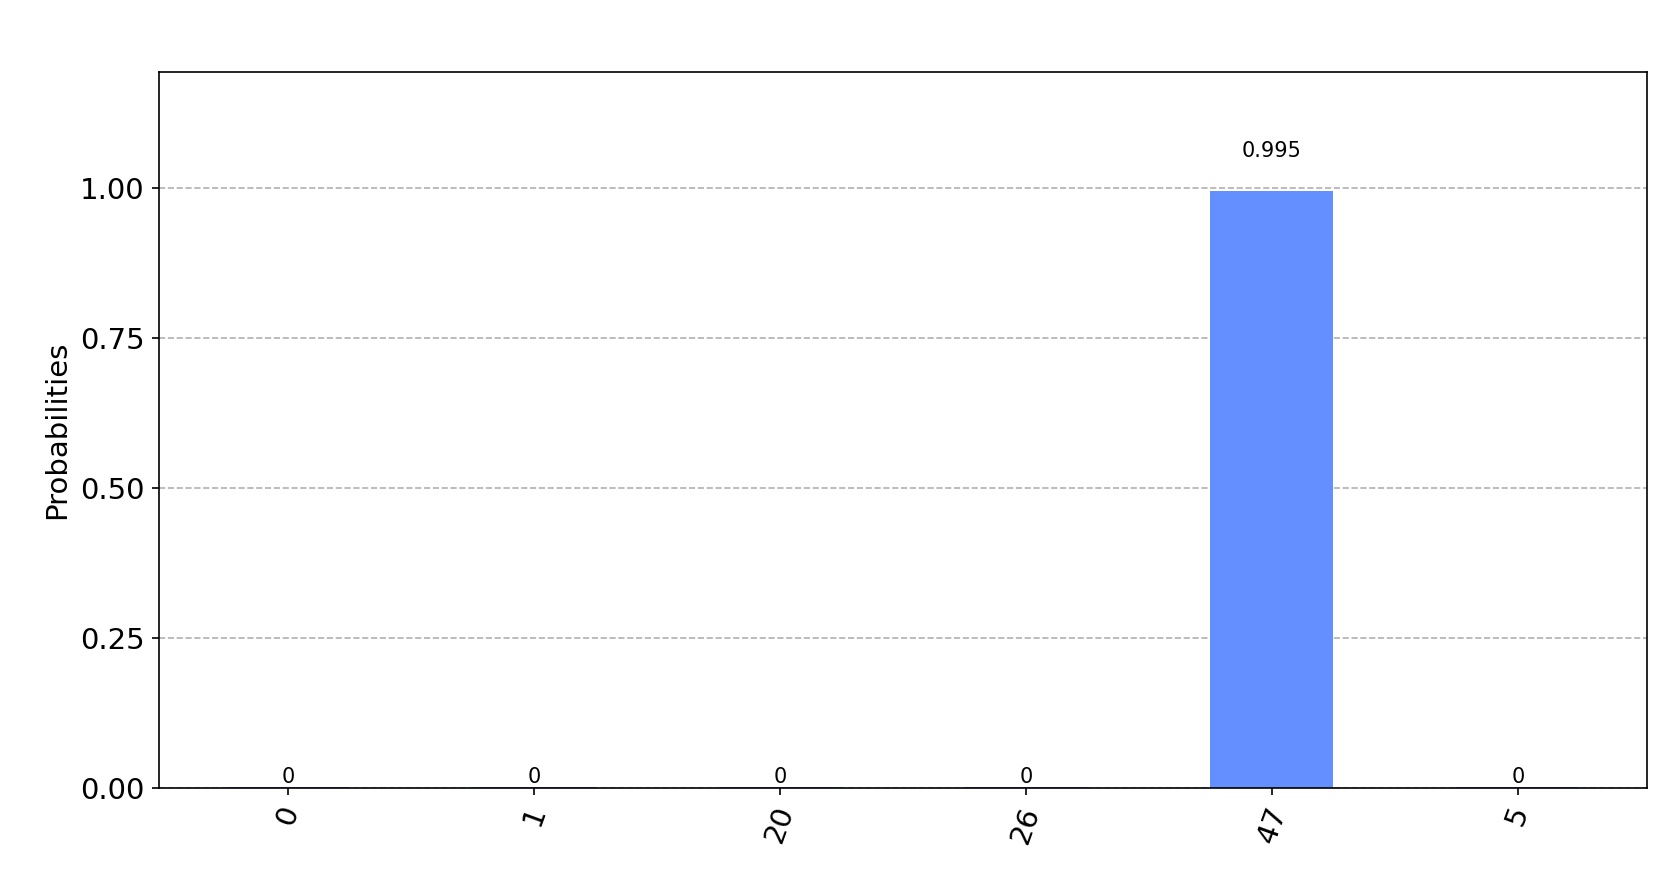
\includegraphics[keepaspectratio, width=15cm, height=15cm]{plot}

We can see that the probability of input 47 is 99.5\%.

\section{Implementation Analysis and Practical Considerations}{}
We are limited when finding a nonce as it may not fit in $n$ bits. We have to know before hand if a solution exists in $n$ bits. There is also another problem, the amount of space required to store the Unitary matrix grows exponentially with the number of input bits. For $n$ bits, the space complexity is $O(2^{2n})$. This is because $n$ bits can be in $2^{n}$ states and our matrix has $2^n * 2^n$ entries. \\

\noindent To put this into perspective, even for $n = 20$ bits (which is only a 7 digit base-10 number at most), we would need a matrix with a trillion rows and columns! This obviously will not scale. To further illustrate the impracticality of this, the most recently mined block (at the time of writing), block 713,463 (found at \url{https://www.blockchain.com/btc/block/713463}) had a nonce of 148,510,277 which in binary, is 28 bits, so using our approach we'd need $2^{56}$ entries in our matrix!\\

\noindent We haven't dug deeply into Qiskit internals but, it may be possible to encode only the values on the diagonal of the matrix and then pass it to Qiskit's \lstinline{g.unitary()}. This way, our space complexity would be $O(2^n)$ which is still quite large, but a significant improvement.

\begin{thebibliography}{12}
\bibitem{1}
\url{https://bitcoin.org/bitcoin.pdf}

\bibitem{2} \url{https://cotinetwork.medium.com/ledgers-over-the-years-from-ancient-
egypt-to-blockchain-dag-and-beyond-47924175cb97}

\bibitem{3} \url{https://github.com/bitcoin/bitcoin/blob/master/src/primitives/block.h#:~:text=//%20header-,int32_t%20nVersion%3B,-uint256%20hashPrevBlock%3B}

\bibitem{4} \url{https://en.wikipedia.org/wiki/Grover%27s_algorithm}
\bibitem{5}  \url{https://www.cnbc.com/2021/06/10/bitcoin-btc-price-jumps-after-el-salvador-adopts-it-as-legal-tender.html}
\bibitem{6} \url{https://www.cnbc.com/2018/03/07/bitcoin-just-tanked-below-10000-after-sec-says-crypto-exchanges-must-register-with-agency.html}
\bibitem{7} \url{https://en.wikipedia.org/wiki/Hashcash}
\bibitem{8} \url{https://www.asicminervalue.com/}
\bibitem{9} \url{https://bitcoin.stackexchange.com/questions/5838/how-is-difficulty-calculated}
\bibitem{10} \url{https://www.nytimes.com/interactive/2021/09/03/climate/bitcoin-carbon-footprint-electricity.html}
\bibitem{11} \url{https://bitcoin.org/en vocabulary#:~:text=Transactions%20receive%20a%20confirmation%20when,for%206%20confirmations%20or%20more.}
\bibitem{12} \url{https://en.bitcoin.it/wiki/Difficulty}
\bibitem{13} \url{https://www.investopedia.com/tech/how-does-bitcoin-mining-work/}
\bibitem{14} \url{https://bitcoin.stackexchange.com/questions/5838/how-is-difficulty-calculated}
\bibitem{15} \url{https://github.com/codebasics/cool_python_apps/blob/main/2_bitcoin_mining/bitcoin_mining.py}
\bibitem{16} \url{https://www.youtube.com/watch?v=5auv_xrvoJk}
\bibitem{17} \url{https://www.investopedia.com/terms/n/nixon-shock.asp}
\end{thebibliography}


\end{document}
